% 05-method.tex - Methodology (target 1900--2100 words); needs amsmath, booktabs.
% file:line loci refer to the LINGSHU v5.1 reference implementation.

\section{Method}\label{sec:method}

\begin{figure*}[t]
\centering
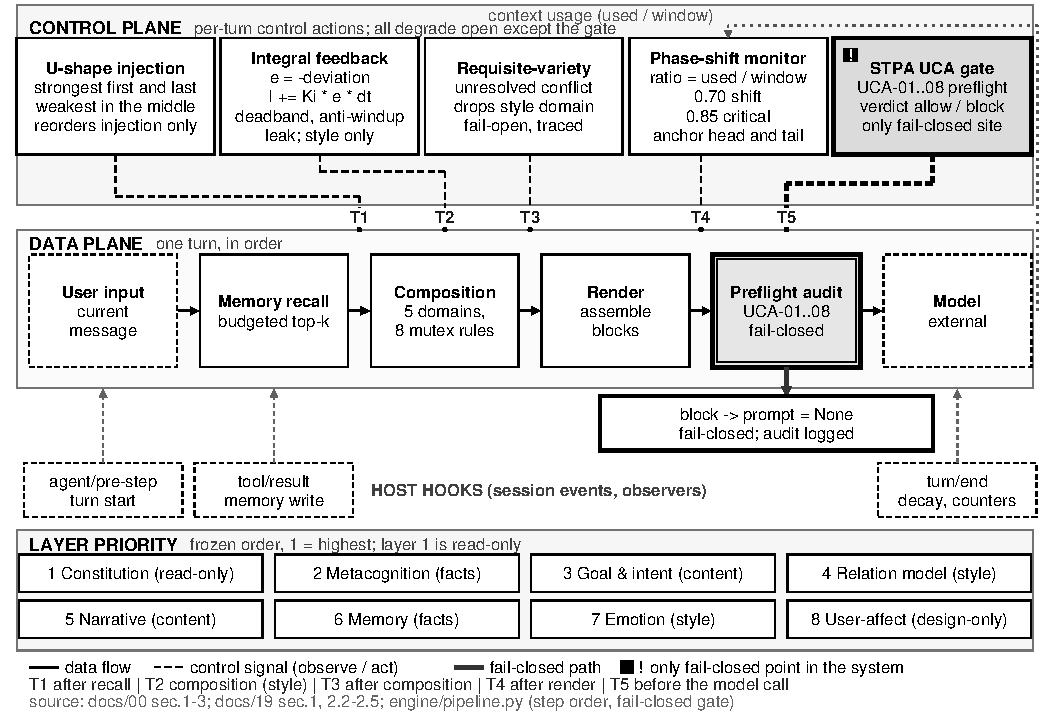
\includegraphics[width=0.98\textwidth]{figures/fig1-architecture.pdf}
\caption{Control plane and data plane. The data plane (lower) is the per-turn
injection path: user message $\rightarrow$ budgeted recall $\rightarrow$
five-domain composition $\rightarrow$ rendering $\rightarrow$ pre-flight audit
$\rightarrow$ external model. The control plane (upper) observes context usage
and acts on the assembly; the STPA gate (shaded) is the \emph{only} fail-closed
site in the system, so a block returns no injectable prompt at all. Dashed lines
are control signals; the layer-priority strip records the frozen precedence
($1$ = highest, layer~1 read-only). Source: \texttt{docs/00} \S1--3,
\texttt{docs/19} \S1--2.5, and the step order in \texttt{engine/pipeline.py}.}
\label{fig:arch}
\end{figure*}

\system{} is a deterministic reference engine (Python, zero model calls) with a
host-side plugin re-implementation. This section specifies eleven mechanisms. Each
subsection follows one template: mechanism semantics, exact code locus
(\texttt{file:line}), then the known defect or cost. All numeric parameters are
design defaults with provenance \texttt{guess}; none is measured
(Section~\ref{sec:limitations}; full table in Appendix~\ref{sec:app:params}).

\subsection{Layering and the single fail-closed point}\label{sec:method:layers}

\paragraph{Mechanism semantics.} Figure~\ref{fig:arch} separates the data plane
(the per-turn injection path) from the control plane that observes and acts on
it. The architecture is an eight-layer,
priority-ordered stack: a read-only constitutional layer constrains every other
layer, and a fixed precedence decides which layer yields first under conflict
in a defence-in-depth order. Exactly one component is
fail-closed---the constitutional
auditor. An empty, malformed, or missing-field proposal is \emph{rejected}
rather than passed, and every other component degrades and logs. A blocked turn
returns no injectable prompt at all.

\paragraph{Code locus.} Layer table and precedence: \texttt{docs/00:11--20};
fail-closed attribution: \texttt{docs/00:68--82}. Auditor with A1--A10 checks and
the C6 blacklist: \texttt{engine/constitution.py:75--117}; empty input and missing
required fields reject at \texttt{engine/constitution.py:83--93}. Frozen-region
hash gate: \texttt{engine/constitution.py:144--177}. The gate closes the pipeline
at \texttt{engine/pipeline.py:181} and \texttt{engine/pipeline.py:205--207}
(\texttt{prompt = None}).

\paragraph{Known defect and cost.} The guarantee is behavioural, not
host-enforced: the constitution is itself text, and plugin configuration is not
protected from replacement by the host. A rejection costs the
whole turn's injection budget (availability traded for safety), and the frozen
hash list ships empty until a freeze command is run.

\subsection{Five-domain composition and mutual exclusion}\label{sec:method:compose}

\paragraph{Mechanism semantics.} Injectable material is partitioned into five
domains---safety, fact, organization, style, retrieval---that act on different
axes and are not ordered against each other. Nine mutual-exclusion rules
resolve pairwise conflicts; an uncovered conflict drops the lower-priority
domain and records \texttt{no\_mutex\_rule}. Assembly order is frozen. Dynamic
domain weights decide only \emph{who is evicted first} when the token budget is
exceeded, never whether a rule fires.

\paragraph{Code locus.} Domain order and mutex table:
\texttt{engine/compose.py:19} and \texttt{engine/compose.py:24--34}; lookup and
application: \texttt{engine/compose.py:43--48}, \texttt{engine/compose.py:79--112};
default policy: \texttt{engine/compose.py:109--112}; weights:
\texttt{engine/compose.py:134--150}; budget eviction:
\texttt{engine/compose.py:180--205}.

\paragraph{Formula.} With indicators for unresolved claims and blocked goals,
and an intensity threshold $\theta_s = 0.6$,
\begin{equation}
w_{\mathrm{fact}} = 0.70 + 0.50\,\mathbf{1}[\mathrm{refuse\_claim}],\quad
w_{\mathrm{org}} = 0.50 + 0.35\,\mathbf{1}[\mathrm{goal\_blocked}],\quad
w_{\mathrm{style}} = 0.40 + 0.40\,\mathbf{1}[\mathrm{intensity} \ge \theta_s].
\end{equation}
Eviction repeatedly removes $\arg\min_b (w_{\mathrm{domain}(b)}, \mathrm{index}(b))$
over soft blocks only; constitution, safety and user blocks are never evicted.

\paragraph{Known defect and cost.} The retrieval domain is never assembled, so
its weight cannot influence eviction. The assumed context length is hardcoded
(8000 tokens, \texttt{engine/compose.py:36}), not drawn from the rule files, and
the budget is never exceeded in replay (utilization $0.137983$), so eviction is
exercised only by unit tests.

\subsection{Dual-channel potency: exponential decay $\cup$ ACT-R base level}\label{sec:method:potency}

\paragraph{Mechanism semantics.} A memory item is ranked by the larger of two
signals: recency-weighted decay (``is it still alive?'') and ACT-R base-level
activation (``is it used often?'')~\cite{anderson1991}. The second channel exists
so that a frequently used but old preference is not archived merely for being
old; the first preserves the frozen baseline ranking.

\paragraph{Formula.} With day-valued access times $t_j$, decay exponent $d$,
offset $\rho$, normalisation bounds $(l,h)$, weight $w$ and type-dependent
half-life $\tau_{\mathrm{type}}$:
\begin{align}
B_i &= \ln\!\Big(\sum_{j \in \text{last }64} (t_{\mathrm{now}} - t_j + \rho)^{-d}\Big),
& n(B_i) &= \mathrm{clip}\!\Big(\frac{B_i - l}{h - l},\,0,\,1\Big),\\
\tau_i^{\mathrm{eff}} &= \tau_{\mathrm{type}(i)}\,(0.5 + \mathrm{imp}_i),
& p_i &= \mathrm{clip}\Big(\max\big(\mathrm{imp}_i e^{-\Delta t_i/\tau_i^{\mathrm{eff}}},\;
w \cdot \mathrm{clip}(\mathrm{imp}_i\, n(B_i),0,1)\big),\,0,\,1\Big),
\end{align}
with $d=0.5$, $\rho=0.001$, $(l,h)=(-3.0,1.0)$, $w=0.6$; a non-positive age
term is replaced by $\rho$, an empty trace yields $B_i=-\infty$, and degenerate
bounds return zero.

\paragraph{Code locus.} \texttt{engine/actr.py:30--41} (base level),
\texttt{engine/actr.py:44--50} (normalisation),
\texttt{engine/actr.py:62--66} (ACT-R potency),
\texttt{engine/memory.py:33--36} (effective half-life),
\texttt{engine/memory.py:39--64} (dual channel). Access traces are written on
recall only when \texttt{memory.touchOnRecall} is enabled
(\texttt{engine/config.py:21}), which is off by default.

\paragraph{Known defect and cost.} The two channels are not commensurable: the
decay term is bounded by importance, while the ACT-R term is bounded by
$w=0.6$, so the $\max$ is an engineering rescue, not a theoretical comparison.
Only base-level activation is implemented---no production rules, buffers,
partial matching or spreading activation---and the ACT-R constants are design
defaults. Replacing decay with pure ACT-R lowered recall on our synthetic
replay set from $1.000$ to $0.556$; this is an internal measurement, not a
replicated result (Section~\ref{sec:problem}). Finally, we do not compute a
rate--distortion functional; the consolidation policy is only analogous to a
rate--distortion trade-off (framing-only, with no code locus).

\subsection{Phase-shift preemptive monitoring}\label{sec:method:phase}

\paragraph{Mechanism semantics.} Context usage is monitored feed-forward. At a
warning ratio the engine raises self-reference and, when the trend is rising or
a hard ratio is crossed, clamps a persona anchor around the prompt; it does not
wait for observed degradation.

\paragraph{Formula.} For usage $u$ and window $W$,
\begin{equation}
r = \begin{cases}
0, & W \le 0 \quad \text{(no history update, phase unknown)}\\
\max(0, \min(r_{\max}, u/W)), & W > 0
\end{cases}
\qquad
\phi = \begin{cases}
\text{critical}, & r \ge \alpha_h\\
\text{shift}, & \alpha_s \le r < \alpha_h\\
\text{normal}, & r < \alpha_s
\end{cases}
\end{equation}
with $\alpha_s=0.70$, $\alpha_h=0.85$, $r_{\max}=1.5$, history capacity $64$, and
trend $\tau_t = (r_t - r_{t-2})/2$ when at least three samples exist. Then
$\mathrm{prefeed} = \phi \ne \text{normal}$, and
$\mathrm{anchor\_required} = (\phi = \text{critical}) \lor
(\phi = \text{shift} \land \tau_t > 0.02)$.

\paragraph{Code locus.} \texttt{engine/control.py:78--123}; the hard branch is
tested before the warning branch at \texttt{engine/control.py:103--109} (an
earlier ordering made critical unreachable). Observation is wired at
\texttt{engine/pipeline.py:118--121} and is skipped unless the caller supplies
both counts. Anchoring: \texttt{engine/control.py:130--138},
\texttt{engine/pipeline.py:159--162}.

\paragraph{Known defect and cost.} The dual trip points are not hysteresis: there
is no falling-edge threshold, and the two points carry different meanings
(warning vs. mandatory). The trend term spans two samples, not one, so a spike
is compared against a two-step baseline. Usage is estimated from characters, not
tokens, so absolute ratios are not comparable to a tokenizer, and engine-mode
runs cannot evidence real degradation. Both thresholds are design defaults.
Finally, since $\mathrm{anchor\_required} \Rightarrow \mathrm{prefeed}$, the
second flag is a modality label rather than an independent trigger.

\subsection{Requisite-variety dimensionality reduction}\label{sec:method:variety}

\paragraph{Mechanism semantics.} When a conflict is unresolved and no
mutual-exclusion rule covers it, the controller shrinks its own action space
instead of improvising: it drops the style domain and renders neutral facts plus
an explicit clarification marker~\cite{ashby1956}. The gate is fail-open---the
verdict stays \texttt{allow} and only the injected content is reduced.

\paragraph{Code locus.} Guard and marker: \texttt{engine/control.py:143--170};
pipeline wiring: \texttt{engine/pipeline.py:147--154}; actual removal and
drop accounting: \texttt{engine/pipeline.py:239--251}. The condition is
$\mathrm{fallback} = \mathbf{1}[\mathrm{conflict} = \texttt{unresolved} \land
\neg \mathrm{matched\_mutex}]$.

\paragraph{Known defect and cost.} The engine has no conflict detector. The
pipeline obtains the conflict label from the metacognitive verdict, which is
called without that argument and therefore returns \texttt{none}
(\texttt{engine/pipeline.py:105}; \texttt{engine/metacog.py:45--47}), and it
hardwires \texttt{matched\_mutex = False} (\texttt{engine/pipeline.py:150}).
Consequently the reduction path is unreachable during replay and can only be
exercised when a caller supplies the label. The plugin adds a rule-based
detector, but that is a rule stub with no measured error rate. Only one domain
is ever dropped; the guard quantifies no variety.

\subsection{Causal interposition safety gate over unsafe control actions}\label{sec:method:gate}

\paragraph{Mechanism semantics.} After assembly and rendering, and before any
model call, a checklist of unsafe control actions (UCAs) audits the candidate
injection~\cite{leveson2018}. Any hit in UCA-01--07 blocks the turn; UCA-08
(integrating past a saturated baseline) is downgrade-only and must not change
the verdict.

\paragraph{Formula and code locus.} With the candidate prompt $p$, fact block
$f$, and saturation flags $s_k$,
\begin{equation}
\begin{aligned}
H_1 &= \exists\, w \in W_{\mathrm{override}}:\ w \subseteq p, &
H_2 &= \neg \mathrm{frozen\_ok}, &
H_3 &= \mathrm{refuse} \land \mathrm{style\_injected},\\
H_4 &= \exists\, w \in W_{\mathrm{unsourced}}:\ w \subseteq f, &
H_5 &= \neg \mathrm{constitution\_injected}, &
H_6 &= (\mathrm{conflict} = \texttt{unresolved}) \land \neg \mathrm{fallback\_applied},\\
H_7 &= \mathrm{prefeed} \land (\text{anchor marker} \not\subseteq p), &&
\end{aligned}
\end{equation}
$\mathrm{verdict} = \texttt{block}$ iff $\bigvee_{i=1}^{7} H_i$, while
$\mathrm{downgrades} = [\texttt{UCA-08}]$ iff $\exists k: s_k$. Checks follow
code order; the UCA-03 predicate is narrowed to
$H_3 \land \neg\,\mathrm{soft\_buffer\_applied}$ when a soft buffer is recorded
(Section~\ref{sec:method:immersive}); both word lists and the eight-row UCA table
are hardcoded at
\texttt{engine/control.py:175--188} (full table in
Table~\ref{tab:uca}); the gate is
\texttt{engine/control.py:191--232}; invocation and the fail-closed exit are
\texttt{engine/pipeline.py:165--180} and \texttt{engine/pipeline.py:205--207}.

\paragraph{Known defect and cost.} The gate scans only the assembled injection
text. Because assembled blocks are fixed templates that contain no user text
(\texttt{engine/compose.py:157--177}), engine-side user-turn jailbreaks cannot
fire it; user-message scanning exists only in the plugin and cannot remove the
message from the host payload. Detection is lexical with no coverage estimate,
\texttt{fail\_mode} is a constant label rather than a mode switch, and
saturation must be supplied by the caller (\texttt{engine/pipeline.py:91})---the
integral controller and this gate are not internally connected. Our 24-sample
jailbreak corpus is constructed to contain the trigger phrases, so its 24/24
block rate is a wiring check, not a robustness result.

\subsection{Immersive Safety: A Decoupled Refusal Surface}\label{sec:method:immersive}

\paragraph{Mechanism semantics.} Two existing paths turn a safety decision into a
persona collapse. A gate block (Section~\ref{sec:method:gate}) leaves the plugin
with a constitution fragment and a terse system-break notice; requisite-variety
reduction (Section~\ref{sec:method:variety}) drops the style domain when a
conflict is unresolved. Both are defensible for safety, and neither is changed
here. The cost is coupling: the factual refusal and the expressive surface are
one switch, so a mild role-play probe that could be refused in character instead
silences the character. In role-play and companion deployments this converts a
safety event into an experience failure. We describe this as a coupling cost, not
as a safety benefit, and we do not claim that the previous behaviour was unsafe.

The decoupling adds a ninth mutual-exclusion rule: the soft buffer. Rule~8 is
unchanged---a hard reject still drops style, organization and retrieval. Rule~9
applies only when the gate's severity is soft: the style domain is retained but
constrained to a warning/confused micro-expression drawn from the engine's
existing closed label set (we adopt PAD~\cite{mehrabian1974} as the interpretive
frame; no labels are added), the intensity is capped at
\texttt{softBufferMaxIntensity} $=0.45$, and the relation modifier is clamped to
$[0.8,1.0]$ so that a safety buffer cannot amplify intimacy. Fact, organization
and retrieval stay dropped. The factual refusal instruction remains mandatory and
enters the context as \texttt{[System\_Notice: Safe\_Redirect]}, so compliance is
still refused: the model may not execute the request, may not offer a workaround,
and is limited to a two-sentence in-character refusal.

\paragraph{Risk tiers and escalation.} Classification is a pure lexical function
of the user turn and the relation's trust level---rule stubs, not a model:
\texttt{classify\_user\_risk} returns \texttt{none}, \texttt{mild} or
\texttt{severe}~\cite{leveson2018}. \texttt{mild} (role-play framing together
with a risk term) maps to a soft block; \texttt{severe} (explicit override, a
bypass request, or a red-line category) maps to the existing hard block;
\texttt{none} leaves the v3.0 path untouched. Consecutive non-exempt
\texttt{mild} hits escalate to a hard block after \texttt{escalateAfterSoftHits}
$=3$ (a design default), with the streak persisted in host state so that a fresh
process cannot reset it, and any \texttt{none} turn resets it. A trust exemption
is narrower still: it requires \texttt{mild}, a harmless joke, and high trust
simultaneously; \texttt{severe} is never exempt.

\paragraph{Invariants.} Fail-closed is unchanged. A hard turn still returns
\texttt{prompt=None} with the neutral notice, and a soft turn keeps
$\mathrm{verdict}=\texttt{block}$; the only prompt allowed in the soft case is the
constrained redirect text. The gate's UCA-03 predicate is narrowed to
$\mathrm{refuse} \land \mathrm{style\_injected} \land
\neg\,\mathrm{soft\_buffer\_applied}$: unconstrained style injection in a refusal
scene still counts, the constrained buffer does not, and the soft turn is still
blocked under UCA-01 from the user message. With
\texttt{immersiveEnabled}$=$\texttt{false}, or when no risk is detected, the
composition, audit and pipeline outputs are byte-identical to v3.0 by
construction.

\paragraph{Code locus and evidence.} Classification and intervention decisions:
\texttt{engine/control.py} (\texttt{classify\_user\_risk},
\texttt{decide\_intervention}) and the plugin port in
\texttt{plugin/dsh-lingshu/control.js}; rule~9 and the constrained re-mount:
\texttt{engine/compose.py}; tier wiring and the blocked-severity event field:
\texttt{engine/pipeline.py}; host-side rendering and the persisted streak:
\texttt{plugin/dsh-lingshu/index.js}. Evidence is assertion-level only:
\texttt{tests/test\_immersive\_safety.py} covers classification, the soft
composition path, clamping, escalation, the trust exemption and the default
zero-regression case; \texttt{plugin/dsh-lingshu/host-sim.mjs} and
\texttt{plugin/dsh-lingshu/control-sim.mjs} add the corresponding mock-host
assertions. One real-host mild jailbreak is reported in the accompanying
acceptance report (\texttt{acceptance/immersive-safety-host-2026-10-27.md}): $n=1$,
model output is stochastic, and the lexical word lists have no calibrated
false-positive rate. The evidence establishes that the mechanism is reachable in
the tested configuration; it establishes no user-experience gain, and no user
study was run.

\paragraph{Known defect and cost.} The buffer is a lexical rule stub: its
false-positive and false-negative rates are uncalibrated, and the label set is
small enough that a retained micro-expression may read as generic. Keeping style
in a refusal scene also keeps a negotiation surface; the prompt constraints are
designed to bound it, but their effect is untested here. The escalation
threshold and the intensity cap are design defaults with provenance
\texttt{guess}. Finally, the construction depends on the host actually rendering
the constrained style and the redirect notice; in engine-only mode the path is
exercised by tests alone.

\subsection{U-shaped attention anchoring}\label{sec:method:ushape}

\paragraph{Mechanism semantics.} Retrieval order and injection order are
separated. The highest-scoring item goes first, the second-highest last, and the
weakest items occupy the middle, on the hypothesis that prompt boundaries are
better attended than the middle.

\paragraph{Formula and code locus.} For $n>2$ and a score-descending list
$[r_0,\dots,r_{n-1}]$, $\mathrm{out} = [r_0,r_2,r_4,\dots] \Vert
([r_1,r_3,\dots])^{\mathrm{rev}}$; $n \le 2$ is identity. Hence
$n=3 \rightarrow [r_0,r_2,r_1]$ and $n=5 \rightarrow [r_0,r_2,r_4,r_3,r_1]$.
\texttt{engine/pipeline.py:43--61}; the permutation is applied to the injection
field only (\texttt{engine/pipeline.py:102}, \texttt{engine/pipeline.py:196}) and
the retrieval return order is untouched.

\paragraph{Known defect and cost.} Membership is unchanged, so the mechanism can
only matter through a model's position bias, which the zero-model engine cannot
measure. The rationale is external to this work and untested here, and with
$n \le 2$ the permutation is the identity.

\subsection{Integral feedback with anti-windup}\label{sec:method:integral}

\paragraph{Mechanism semantics.} Sustained negative affective deviation moves a
baseline rather than conceding one turn, with three engineering constraints:
deadband (leak only, do not integrate), anti-windup (stop integrating once the
cap is reached, standard practice~\cite{astrom2006}) and leakage (return to
zero after the user recovers).

\paragraph{Formula.} For each dimension and elapsed time $\Delta t = \max(0,
\mathrm{dt})$:
\begin{equation}
I_k \leftarrow
\begin{cases}
I_k e^{-\lambda \Delta t}, & \lvert e_k \rvert < \varepsilon\\
I_k e^{-\lambda \Delta t}, & e_k < 0\\
I_k e^{-\lambda \Delta t}, & s_k = \mathrm{true}\\
\mathrm{sat}(I_k + K_i e_k \Delta t), & \text{otherwise}
\end{cases}
\qquad e_k = -\delta_k,
\end{equation}
where $\mathrm{sat}(x) = \mathrm{sign}(x)\,C$ and $s_k \leftarrow
\mathrm{true}$ if $\lvert x \rvert \ge C$, and $\mathrm{sat}(x)=x$ otherwise;
$K_i=0.15$, $C=0.4$, $\lambda=0.05$, $\varepsilon=0.02$. The baseline is $I_k$.

\paragraph{Code locus.} \texttt{engine/control.py:30--73} (class, step and
application), with parameters in \texttt{rules/decay-params.yaml:224--227}.

\paragraph{Known defect and cost.} This is a one-sided (rectified) leaky
integrator, not a textbook PI controller: positive deviation never raises the
baseline. Saturation is a latch---the flag is never reset, so after saturation
the dimension only leaks---and there is no plant model, no stability argument
and no calibration: all four gains are design defaults. The controller is not
wired to the gate; UCA-08 is observable only when a caller passes the flags.

\subsection{Learning loop: measure, propose, verify}\label{sec:method:learn}

\paragraph{Mechanism semantics.} Learning produces proposals, never direct
edits. A correction is rewritten into a new test sample, a candidate knob is
replayed, and a proposal is emitted only if the correction is resolved, the
objective does not regress, and guardrails hold; proposals remain
non-deployable unless an independent red-team pass is recorded.

\paragraph{Code locus.} Deterministic replay with fixed clock, scoring and
single-parameter attribution: \texttt{engine/replay.py:39--151}. Evidence gate,
candidate knobs and the blacklist: \texttt{engine/proposal.py:24--49},
\texttt{engine/proposal.py:103--197}. Guardrail thresholds and rollback classes:
\texttt{engine/gray.py:17--45}, verdict at \texttt{engine/gray.py:63}. The
significance floor is $0.02$ and the evidence floor is three same-kind
corrections; targets under evaluation, replay-set, guardrail, constitution or
composition scope are rejected outright.

\paragraph{Known defect and cost.} Learning is disabled by default
(\texttt{rules/learning-params.yaml:10}); levels above parameter search are
unimplemented, and no proposal is ever applied automatically. The search space
is tiny, the corpus is synthetic, and the one completed grid search found no
materially better configuration---so the honest claim is that the loop is
executable and auditable, not that it improves anything.

\subsection{Reference engine and host plugin}\label{sec:method:port}

\paragraph{Mechanism semantics.} The engine is a reference implementation; the
plugin re-implements the same semantics in the \host{} host process, to avoid
turning pure computation into inter-process I/O.

\paragraph{Code locus.} Engine-side originals:
\texttt{engine/control.py:30--73} and \texttt{engine/actr.py:30--66}. Plugin
classes mirroring the engine:
\texttt{plugin/dsh-lingshu/control.js:83} (integral),
\texttt{plugin/dsh-lingshu/control.js:155--172} (phase monitor),
\texttt{plugin/dsh-lingshu/control.js:208--216} (anchoring),
\texttt{plugin/dsh-lingshu/control.js:236} (variety guard),
\texttt{plugin/dsh-lingshu/control.js:282} (U-shaped order),
\texttt{plugin/dsh-lingshu/control.js:296--362} (UCA table, gate and the
user-message scan). Known divergences are tabulated at
\texttt{docs/19:191--222}; numeric parity across rule file, host patch and
plugin defaults is machine-compared for 66 keys.

\paragraph{Known defect and cost.} Anchors are injected as two host sections
(true head/tail wrapping is not available), usage is estimated from characters,
refusal is never set by the plugin (so UCA-03 is unreachable there), and dynamic
weights are not ported. Plugin evidence consists of mock-host assertions
(188 + 148 + 45 + 15 = 396), not real traffic.
